%%% Laboratory	 Notes
%%% Template by Mikhail Klassen, April 2013
%%% Contributions from Sarah Mount, May 2014
\documentclass[a4paper]{tufte-handout}

\newcommand{\workingDate}{\textsc{Mar. $|$ 2023}}
\newcommand{\userName}{\AE ther Zhou}
% \newcommand{\institution}{Your University}

\usepackage{lab_notes}
\usepackage{siunitx}

\usepackage{hyperref}
\hypersetup{
    pdffitwindow=false,            % window fit to page
    pdfstartview={Fit},            % fits width of page to window
    pdftitle={Lab notes 2014},     % document title
    pdfauthor={Your Name},         % author name
    pdfsubject={},                 % document topic(s)
    pdfnewwindow=true,             % links in new window
    colorlinks=true,               % coloured links, not boxed
    linkcolor=DarkScarletRed,      % colour of internal links
    citecolor=DarkChameleon,       % colour of links to bibliography
    filecolor=DarkPlum,            % colour of file links
    urlcolor=DarkSkyBlue           % colour of external links
}


\title{PHYS 128AL Lab Notebook}
\author[]{\AE ther Zhou}
\date{Mar. 2023}

\begin{document}
\maketitle
%%%%%%%%%%%%%%%%%%%%%%%%%%%%%%%%%%%%%%%%%%%%%%%%%%%%%%%%

\begin{projects}
	\begin{description}
        \item [Lab 4] Cloud Chamber 
		\item [Collaborator] Lucas Watkins
		\end{description}
\end{projects}

%%%%%%%%%%%%%%%%%%%%%%%%%%%%%%%%%%%%%%%%%%%%%%%%%%%%%%%%
\tableofcontents

\newpage

%%%%%%%%%%%%%%%%%%%%%%%%%%%%%%%%%%%%%%%%%%%%%%%%%%%%%%%%
\section{Lab Manuel Questions}

\textit{What is the saturation vapor pressure of your alcohol at room temperature?}

According to \url{https://www.sciencedirect.com/topics/engineering/isopropyl-alcohol#:~:text=Molecular\%20weight\%3D60.11\%3B\%20specific\%20gravity,autoignition\%20temperature\%3D399\%C2\%B0C} , at room temperature, the saturation vapor pressure of our isopropyl alcohol in air is 4.40 kPa.

\hrulefill

%%%%%%%%%%%%%%%%%%%%%%%%%%%%%%%%%%%%%%%%%%%%%%%%%%%%%%%%
\textit{At -35C?}

 By Clausius-Clapeyron equation, 
 $$P = Ae^{\Delta H_{vap} / RT}$$

Plugging in $\Delta H_{vap} =  45 \,\si{kJ/mol}$ for isopropyl alcohol, we get $P = $ 0.062 kPa. 

\hrulefill

%%%%%%%%%%%%%%%%%%%%%%%%%%%%%%%%%%%%%%%%%%%%%%%%%%%%%%%%
\textit{If you take 1 cc of saturated gas at room temperature, and chill it to -35,\\ what volume of alcohol needs to condense?}

Ideal gas law 
$$PV = nRT$$
given
\begin{align*}
    P_1 &= 4.4 \,\si{kPa,}\quad V_1 = 1 \,\si{cc,}\quad T_1 = 293.15 \,\si{K}\\
    P_2 &= 0.062 \,\si{kPa,}\quad T_2 = 238.15 \,\si{K}
\end{align*} 
Hence, by
$$P_1 V_1/ T_1 = P_2 V_2/ T_2$$
We solved $V_2 = 0.797 \,\si{cc}$, so $.203$ cc of alcohol needs to condense.


\hrulefill

%%%%%%%%%%%%%%%%%%%%%%%%%%%%%%%%%%%%%%%%%%%%%%%%%%%%%%%%
\textit{Can you use this knowledge, and observation of the density of droplets, to guesstimate the volume of each drop?}

Based on this approximation, we can estimate that approximately 20\% of the gaseous alcohol that was initially introduced into the chamber must condense in order to reach equilibrium. Since we added approximately 10-20 cc of alcohol to the chamber, we can assume that about 1-2 cubic centimeters of alcohol will condense.

\hrulefill

%%%%%%%%%%%%%%%%%%%%%%%%%%%%%%%%%%%%%%%%%%%%%%%%%%%%%%%%
\textit{Particles through matter:}

The alpha particle's electric field possesses sufficient strength to ionize certain gas molecules, resulting in a retarding force that causes a decrease in the energy and velocity of the ionized electron. The frequency of ionization events affects the rate at which the alpha particle slows down, with higher instances of ionization leading to more rapid deceleration. The quantity dE/dx refers to the energy lost per unit distance traveled, with denser gas containing more molecules and consequently resulting in a greater number of collisions that ultimately cause the alpha particle to come to a halt more quickly.

\hrulefill

%%%%%%%%%%%%%%%%%%%%%%%%%%%%%%%%%%%%%%%%%%%%%%%%%%%%%%%%
\textit{Bethe formula:}

$$-\left<\frac{dE}{dx}\right> = \frac{4\pi}{m_ec^2}\cdot\frac{nz^2}{\beta^2}\cdot\left(\frac{e^2}{4\pi\epsilon_0}\right)^2\cdot\left[\ln\left(\frac{2m_ec^2\beta^2}{I\cdot(1-\beta^2)}\right)-\beta^2\right]$$

\hrulefill

%%%%%%%%%%%%%%%%%%%%%%%%%%%%%%%%%%%%%%%%%%%%%%%%%%%%%%%%
\textit{Multiple scattering:}

$$\theta_0 = \frac{13.6 \,\si{MeV}}{\beta cp}z \sqrt{\frac{x}{X_0}}\left[1+0.038\ln{\left(\frac{x}{X_0}\right)}\right]$$
$$X_0 = (1433 \,\si{g cm^{-2}})\frac{A}{Z(Z+1)(11.319-\ln{Z})}$$
\hrulefill

%%%%%%%%%%%%%%%%%%%%%%%%%%%%%%%%%%%%%%%%%%%%%%%%%%%%%%%%
\newpage

%%%%%%%%%%%%%%%%%%%%%%%%%%%%%%%%%%%%%%%%%%%%%%%%%%%%%%%%
\section{Daily}
\newday{6 Mar 2023, M}
Setup of the Cloud Chamber lab (cloud chamber, voltage supply, cooler, CF$_4$ gas)
\\
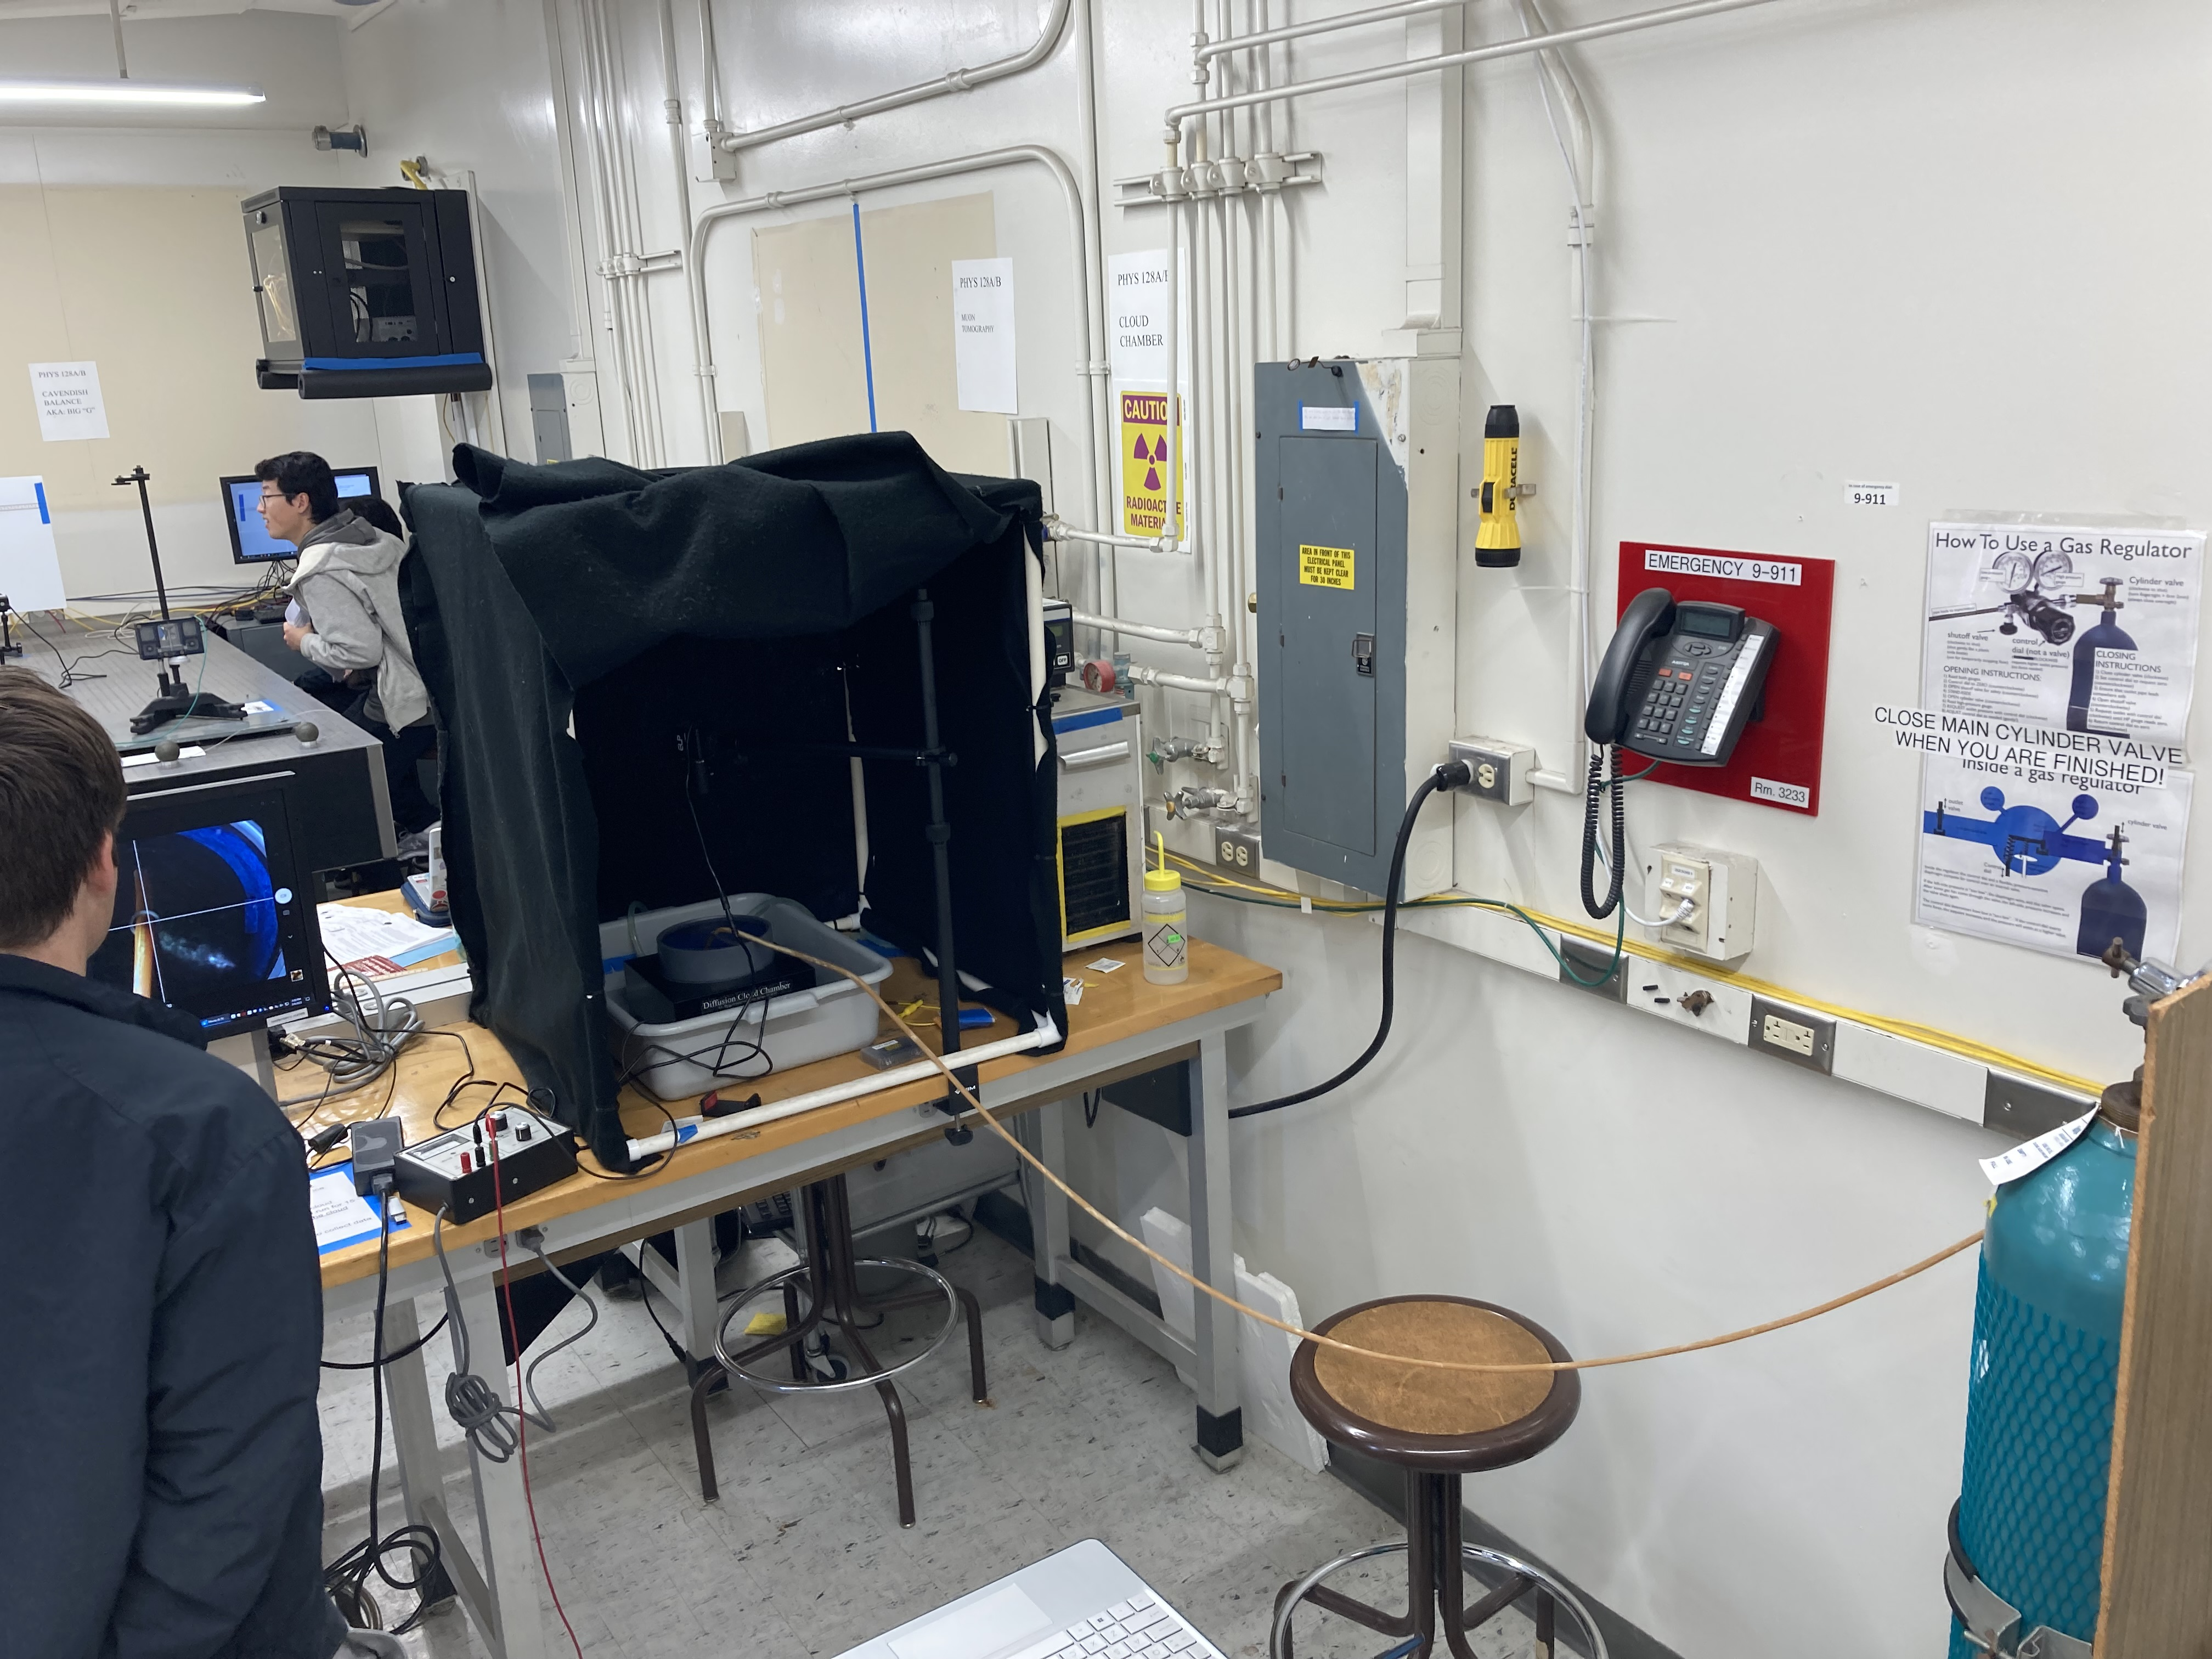
\includegraphics[width = 1 \textwidth]{figures/day1_setup.JPG}
\\
A brief sketch of the chamber structure
\\
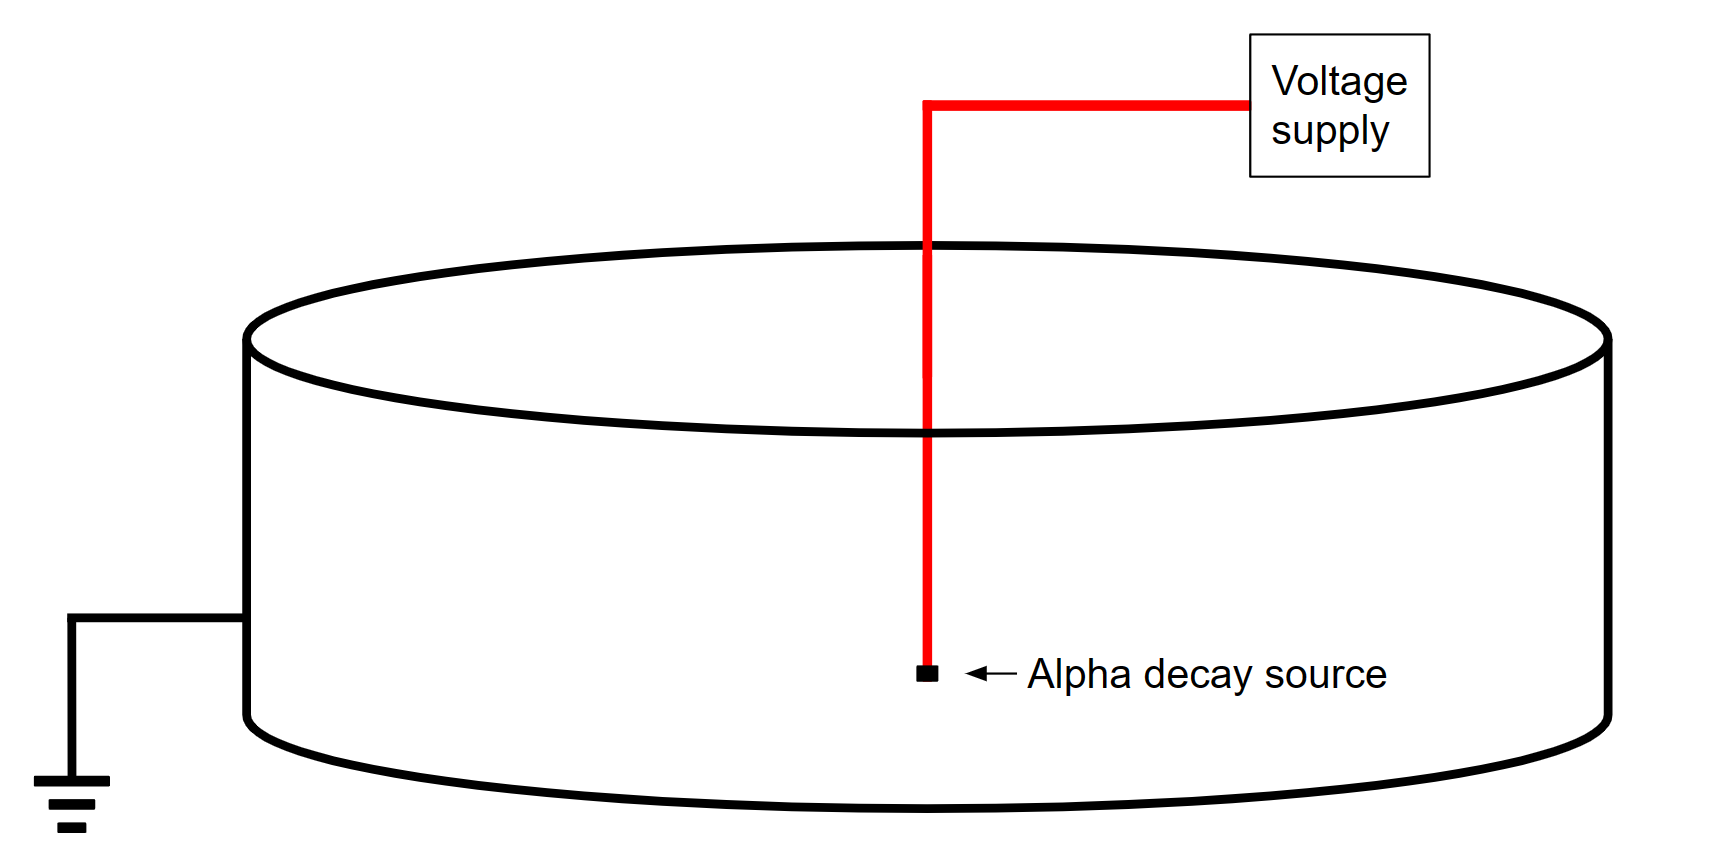
\includegraphics[width = 1 \textwidth]{figures/day1_chamber.png}
\\
Alpha decay observed
\\
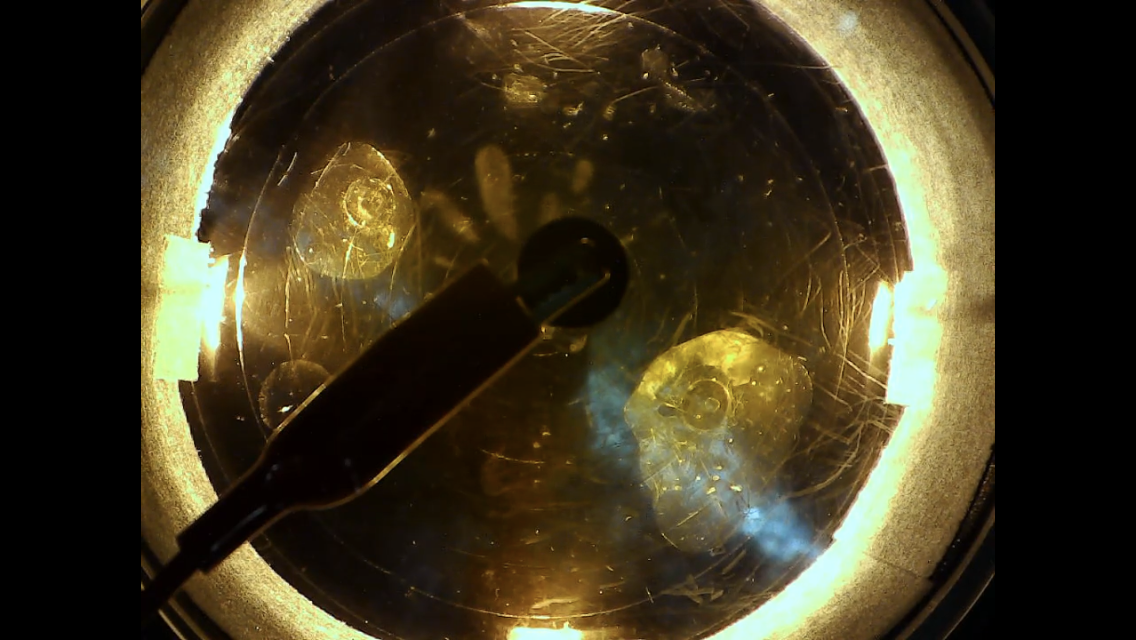
\includegraphics[width = 1 \textwidth]{figures/day1_trajectory.PNG}
\\
\hrulefill

%%%%%%%%%%%%%%%%%%%%%%%%%%%%%%%%%%%%%%%%%%%%%%%%%%%%%%%%

\newday{8 Mar 2023, W}
Measurement of trajectories length, which is assumed to form a Gaussian distribution
\\
Using air as medium, temperature cooled down to $-10$ Celsius, applying voltage difference of $400$ volt
\\
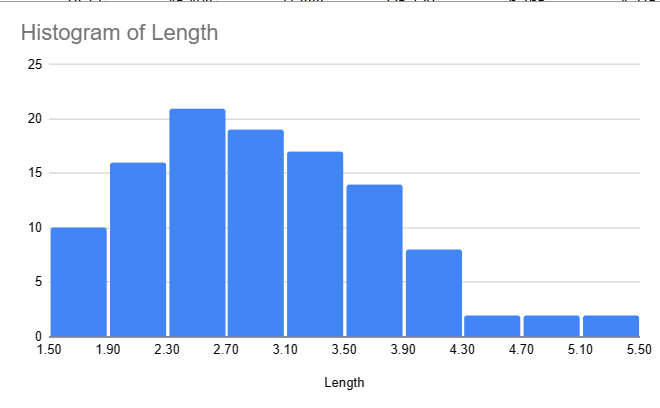
\includegraphics[width = 1 \textwidth]{figures/day2_air400.png}
\\
air, 100 volt; we see less trajectories
\\
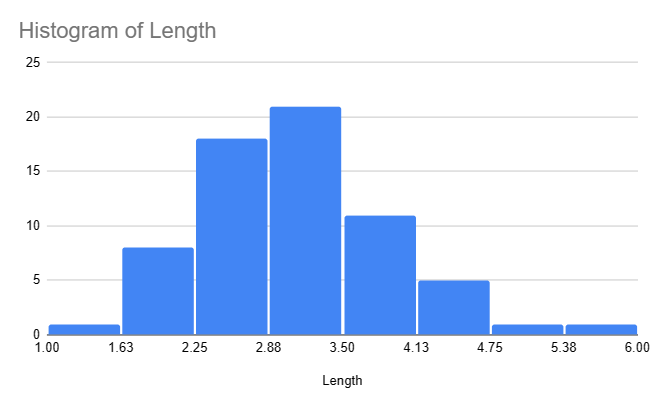
\includegraphics[width = 1 \textwidth]{figures/day2_air100.png}
\\
we filled the chamber with CF$_4$, voltage difference kept at $400$ volt; we see less and shorter trajectories
\\
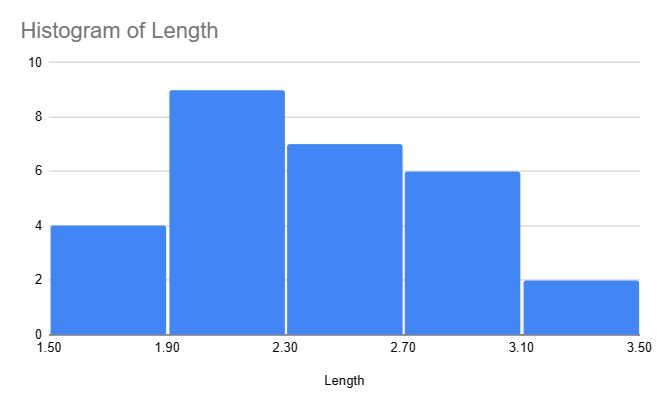
\includegraphics[width = 1 \textwidth]{figures/day2_cf4400.png}
\\
\hrulefill

%%%%%%%%%%%%%%%%%%%%%%%%%%%%%%%%%%%%%%%%%%%%%%%%%%%%%%%%
\newday{13 Mar 2023, M}
Due to high humidity in air, our cloud chamber accumulated enough moisture to form frost.
\\
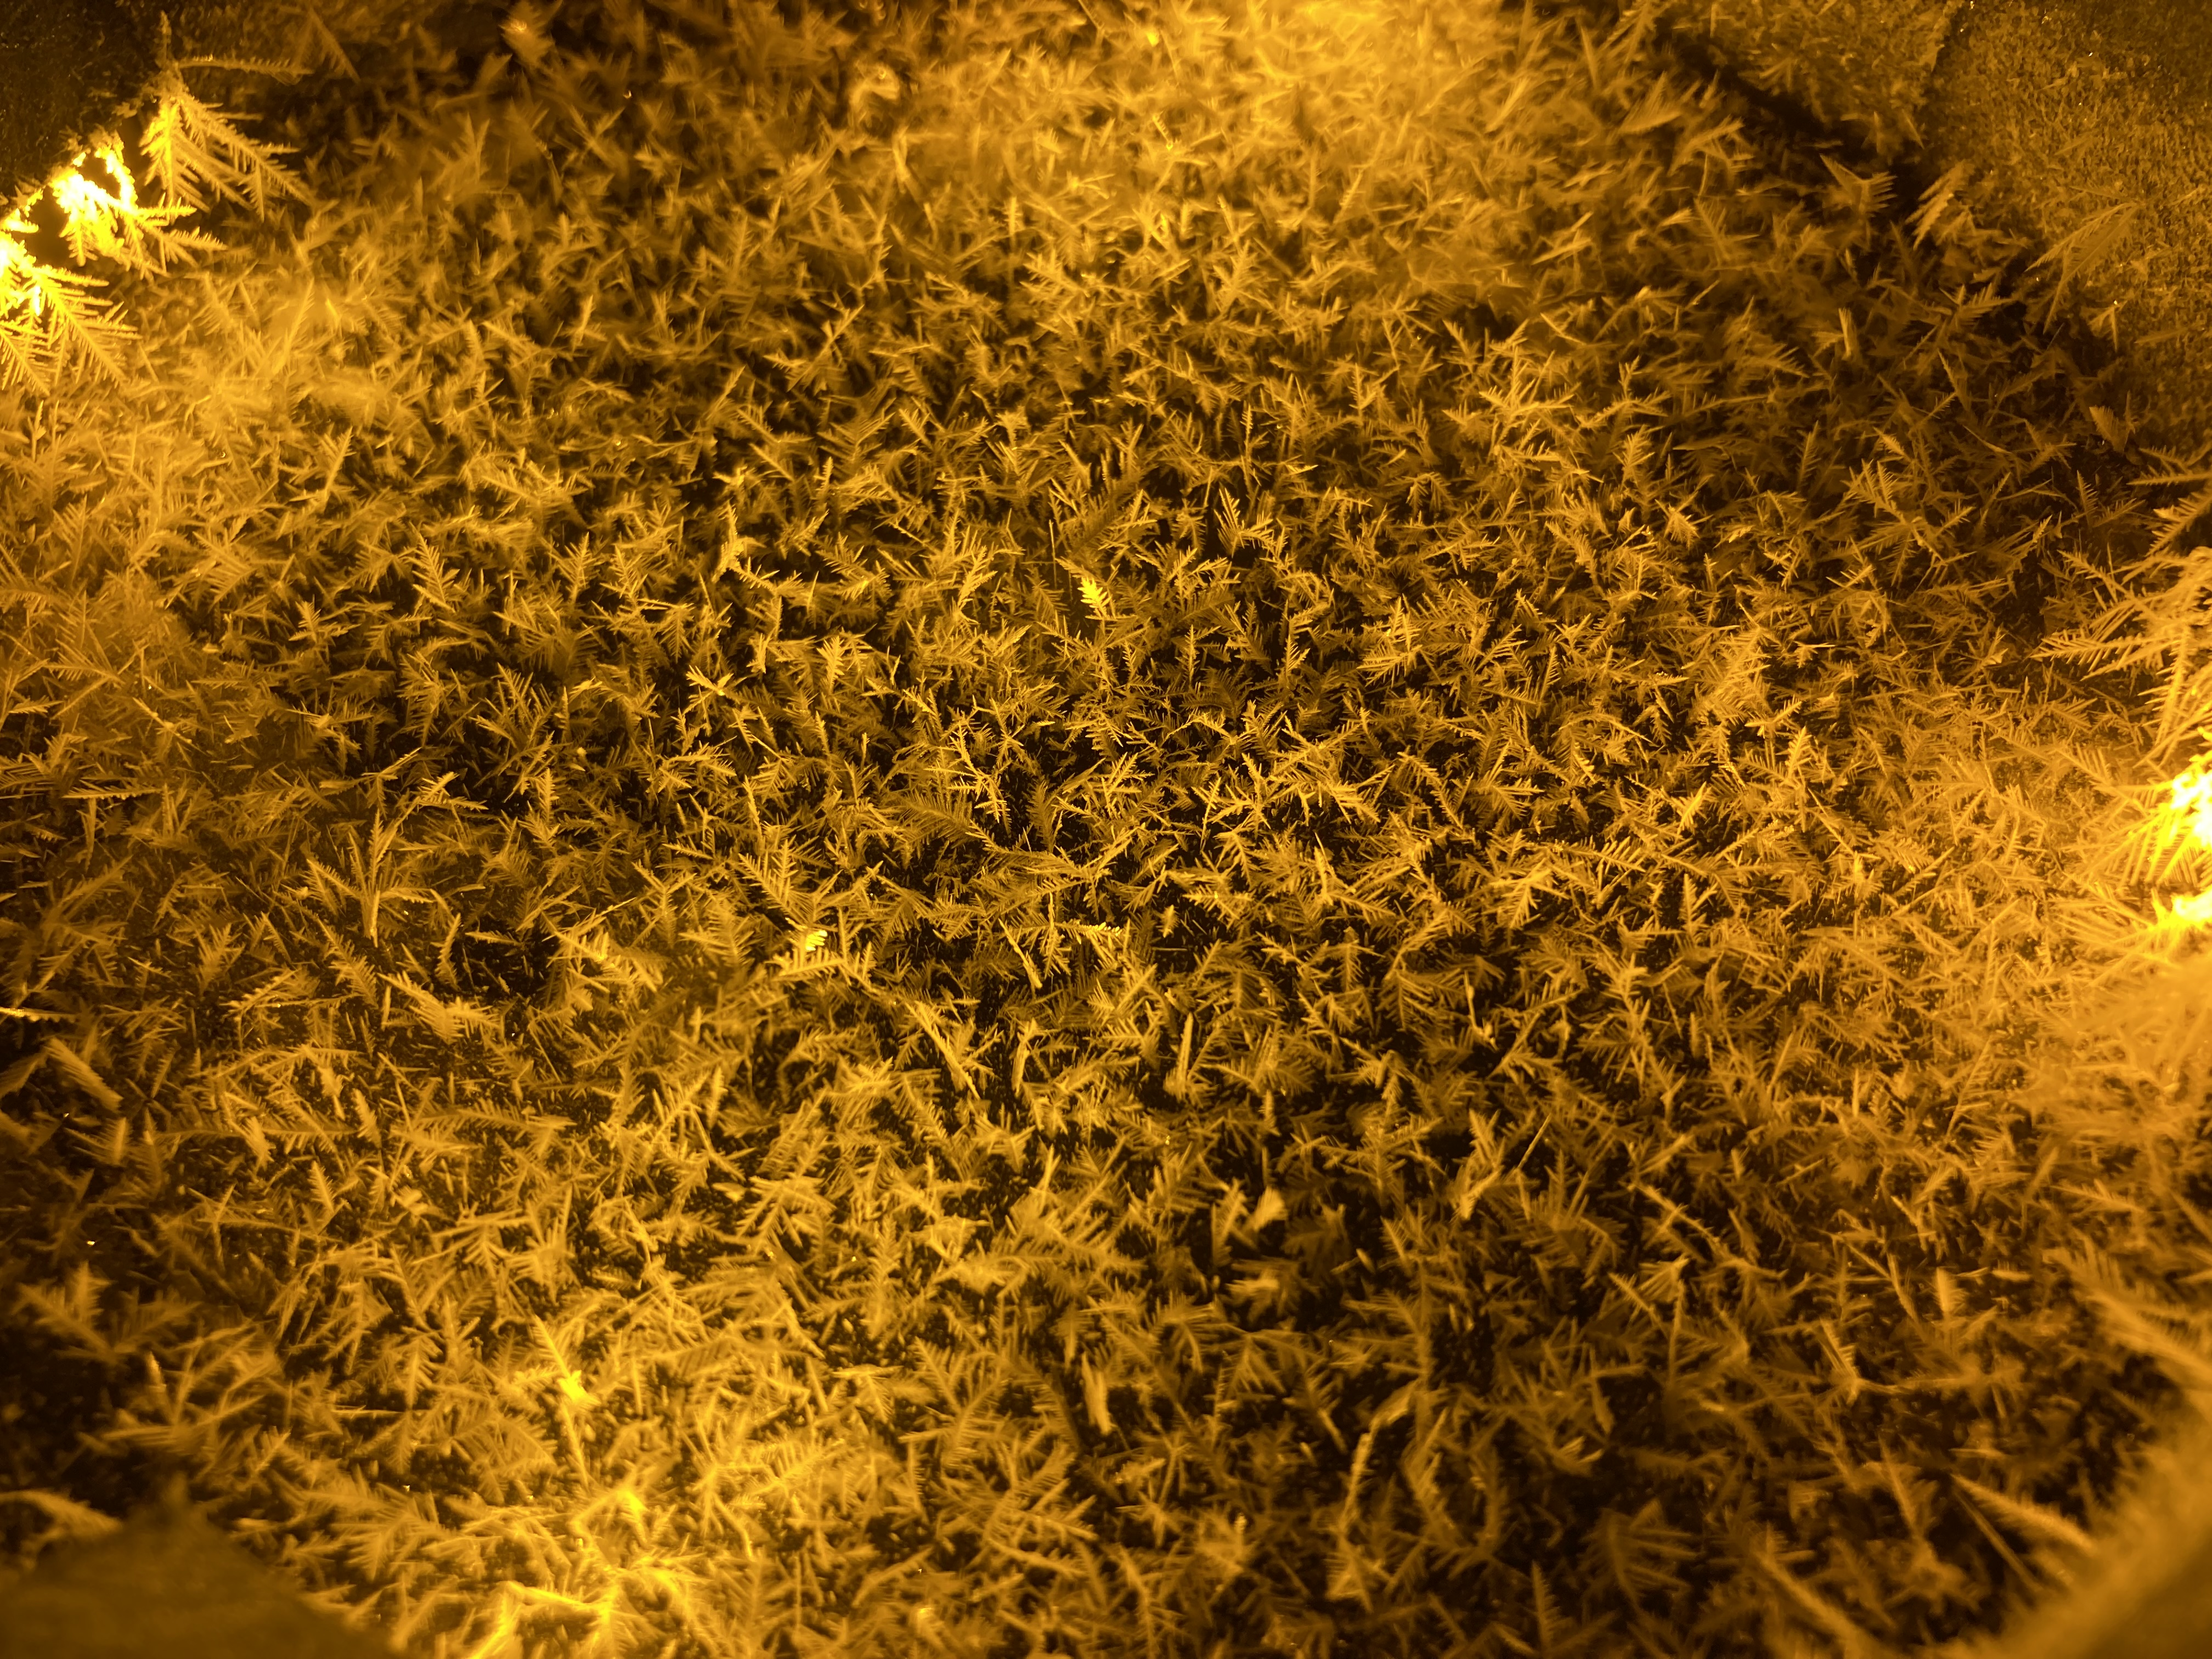
\includegraphics[width = 1 \textwidth]{figures/day3_frost.JPG}
\\
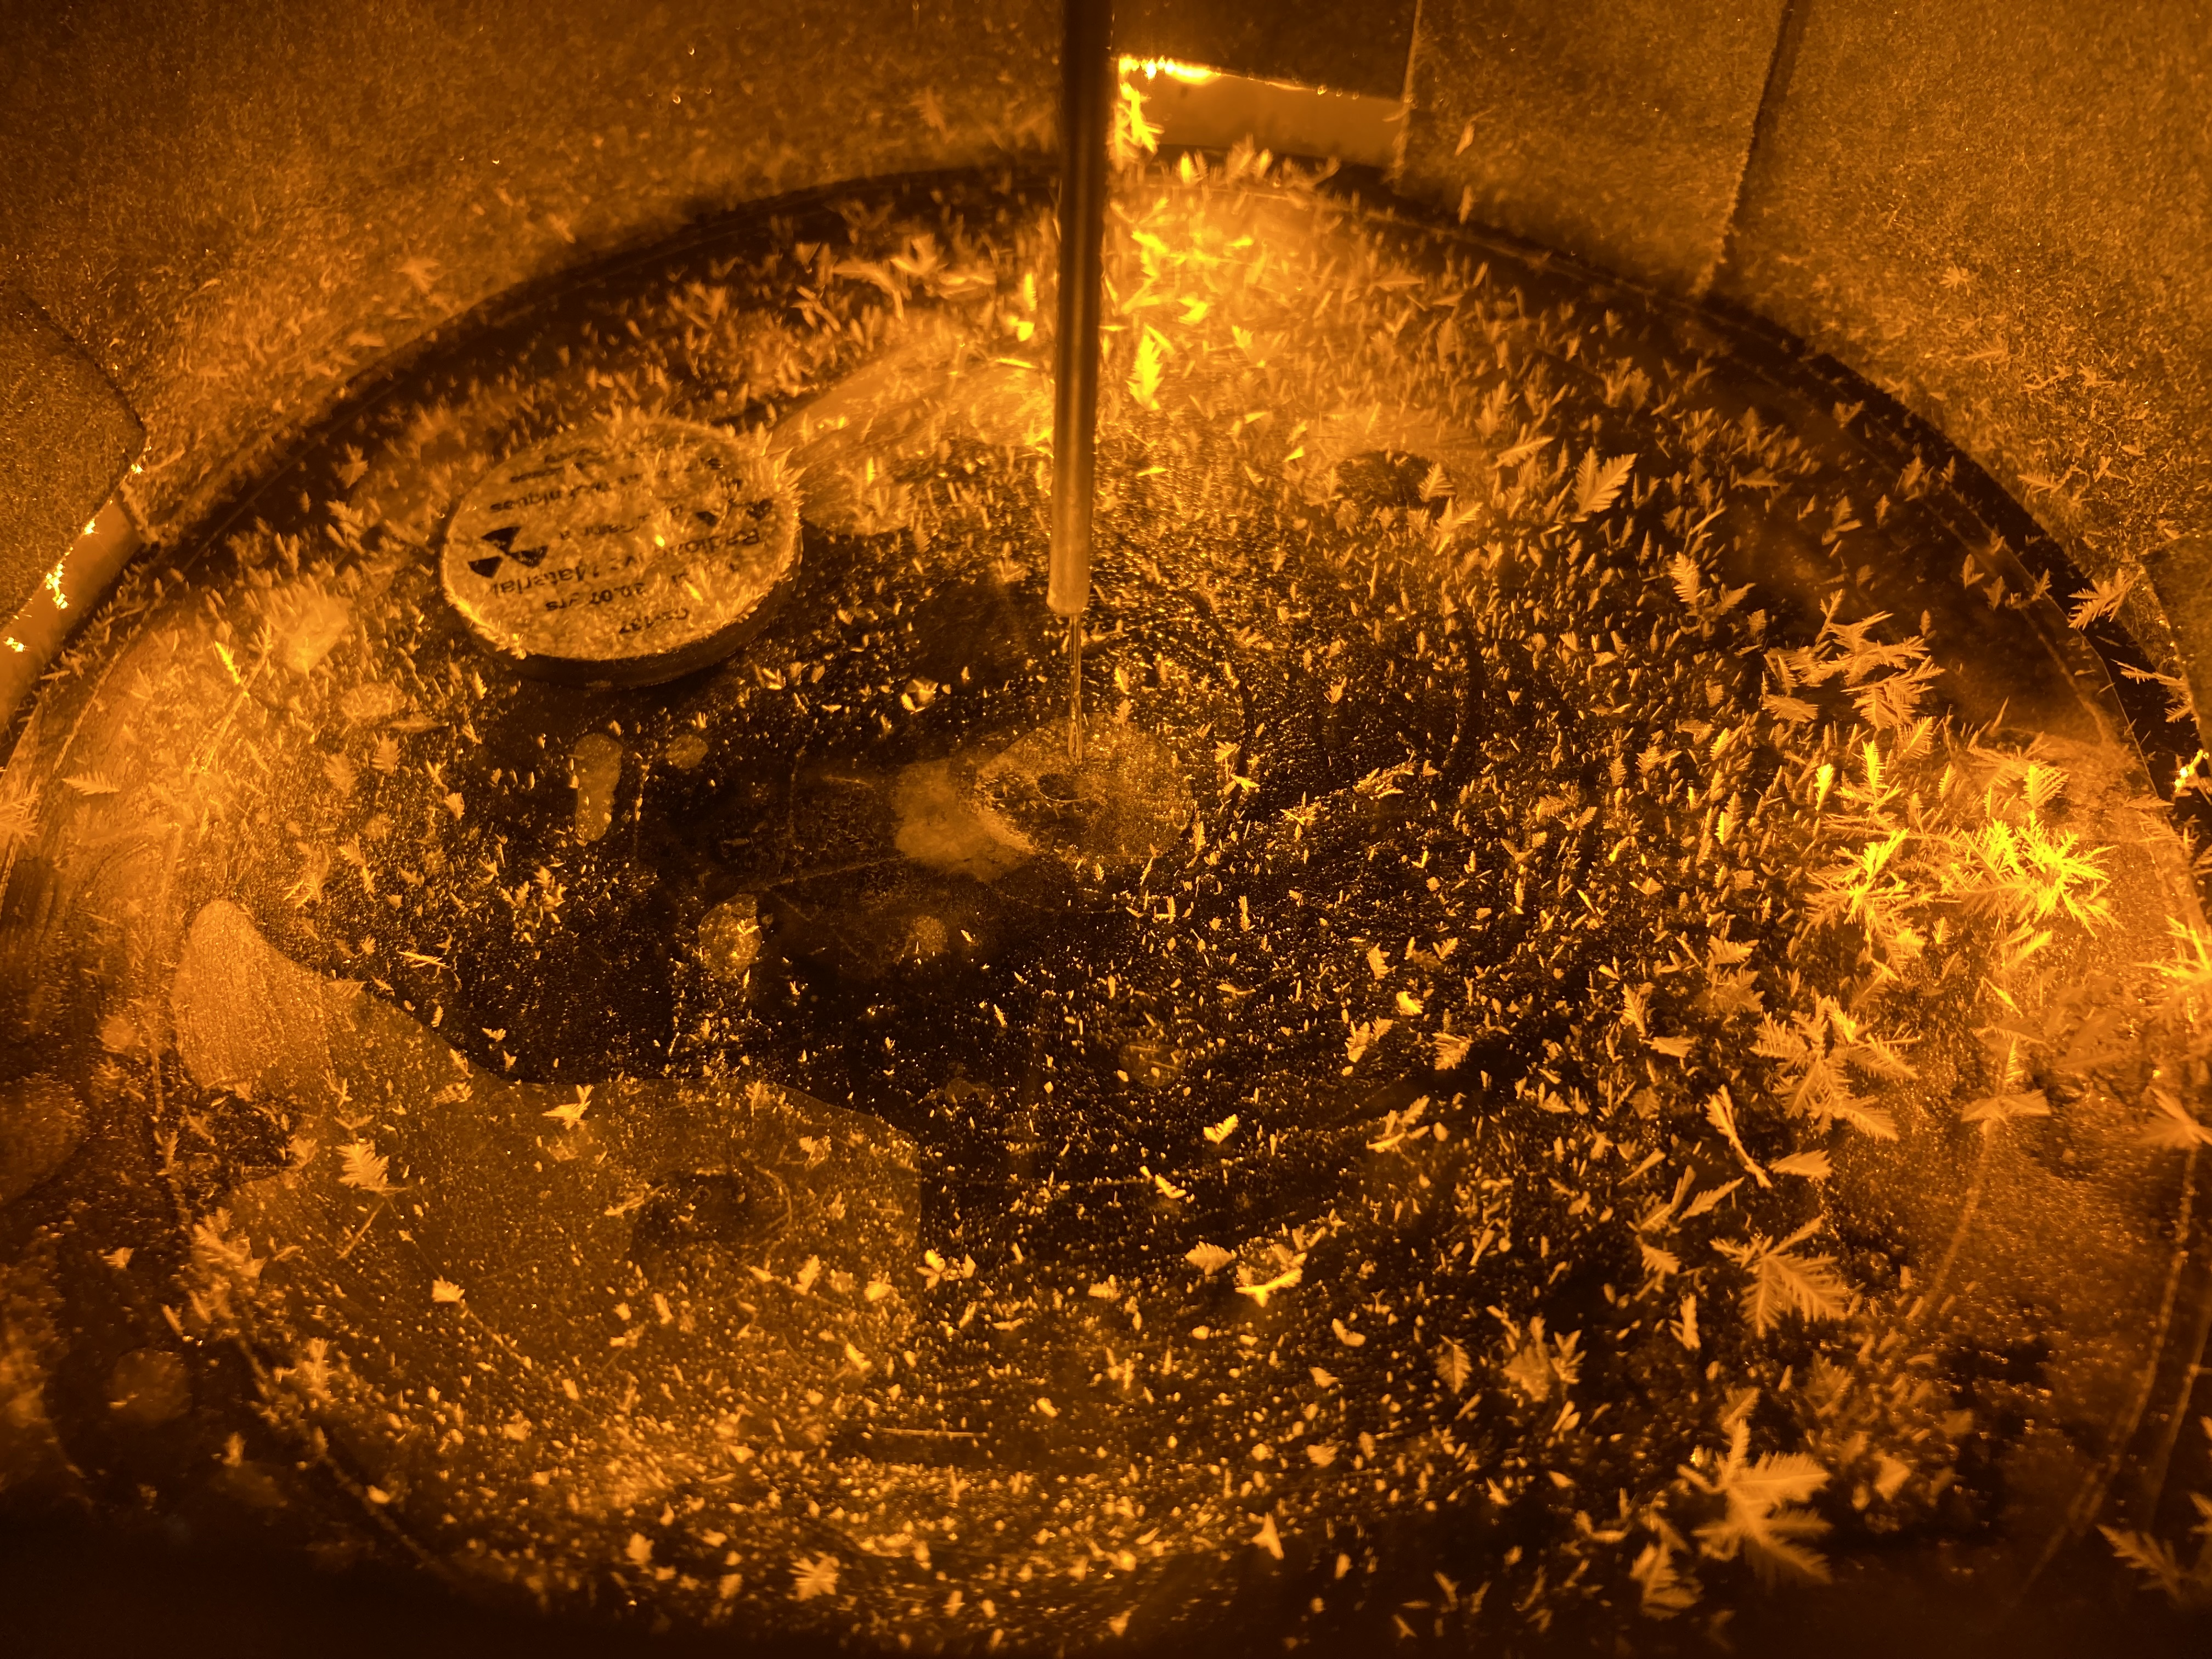
\includegraphics[width = 1 \textwidth]{figures/day3_frost_gamma.JPG}
\\
so we decided to measure the bending angle of trajectories from our video taken on day 2.
\\
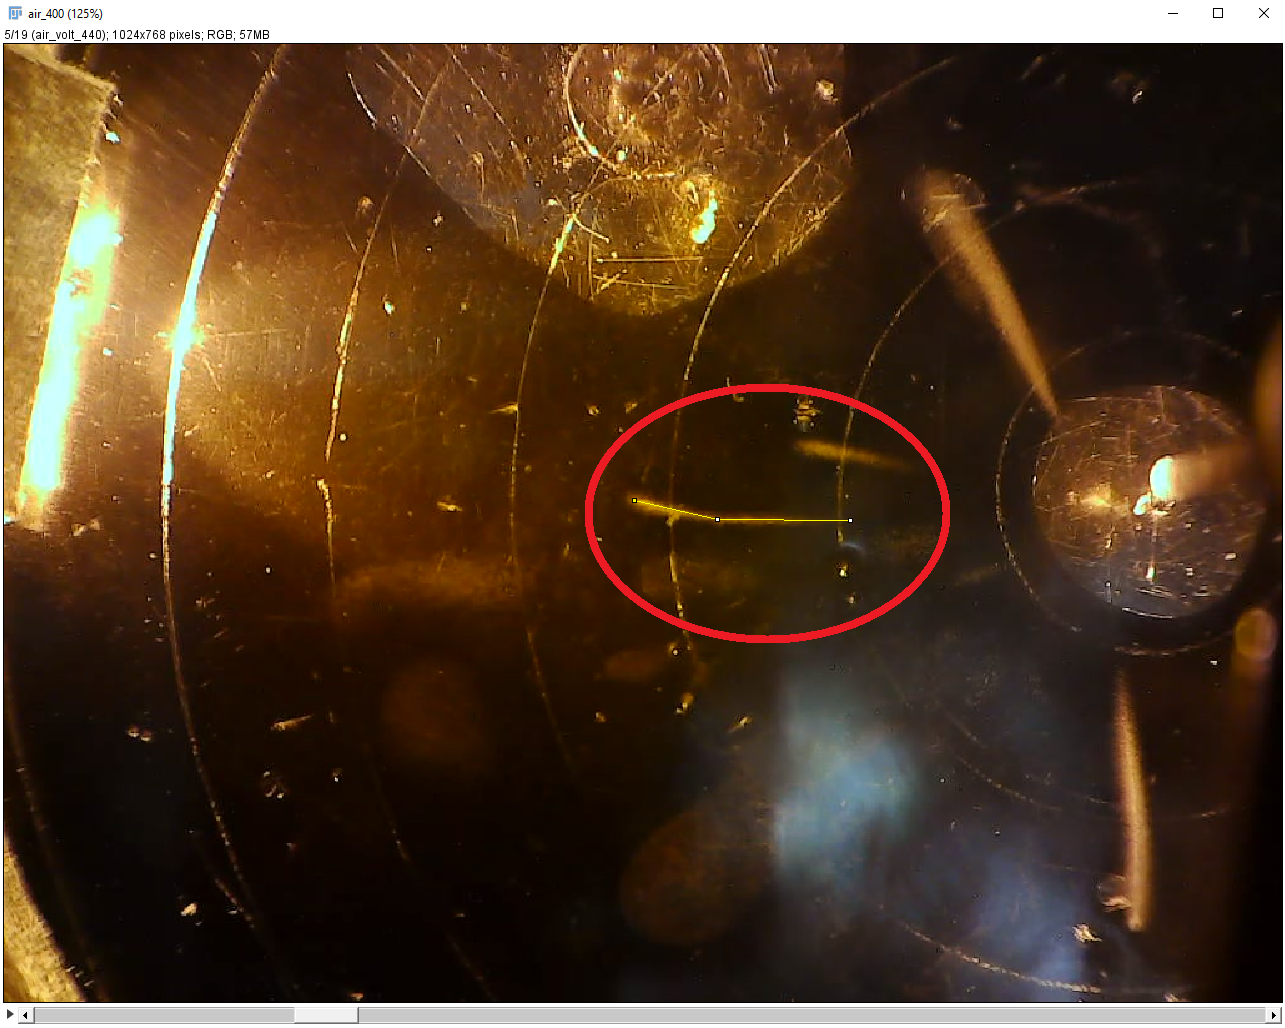
\includegraphics[width = 1 \textwidth]{figures/day3_bends.png}
\\
We measured with ImageJ, similar to what we did for length measurement. Following is the data
\\
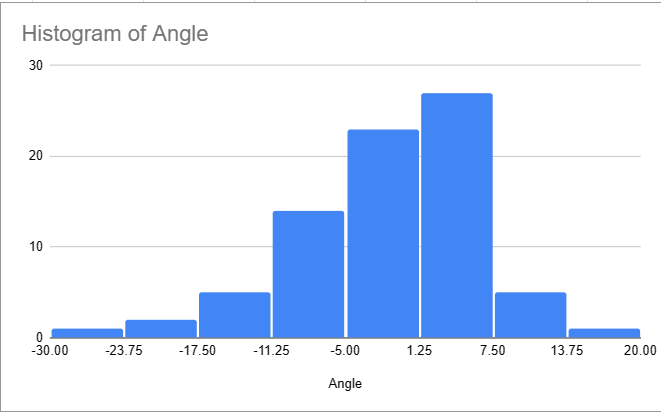
\includegraphics[width = 1 \textwidth]{figures/day3_scat.png}
\\
\hrulefill

%%%%%%%%%%%%%%%%%%%%%%%%%%%%%%%%%%%%%%%%%%%%%%%%%%%%%%%%
\newday{15 Mar 2023, W}
We fitted Gaussian to our data, and discussed on possible cause of errors. Plots are presented under the Result and Analysis section. 

\newpage
\section{Theory and Setup}

\subsection{Set up and Procedure}

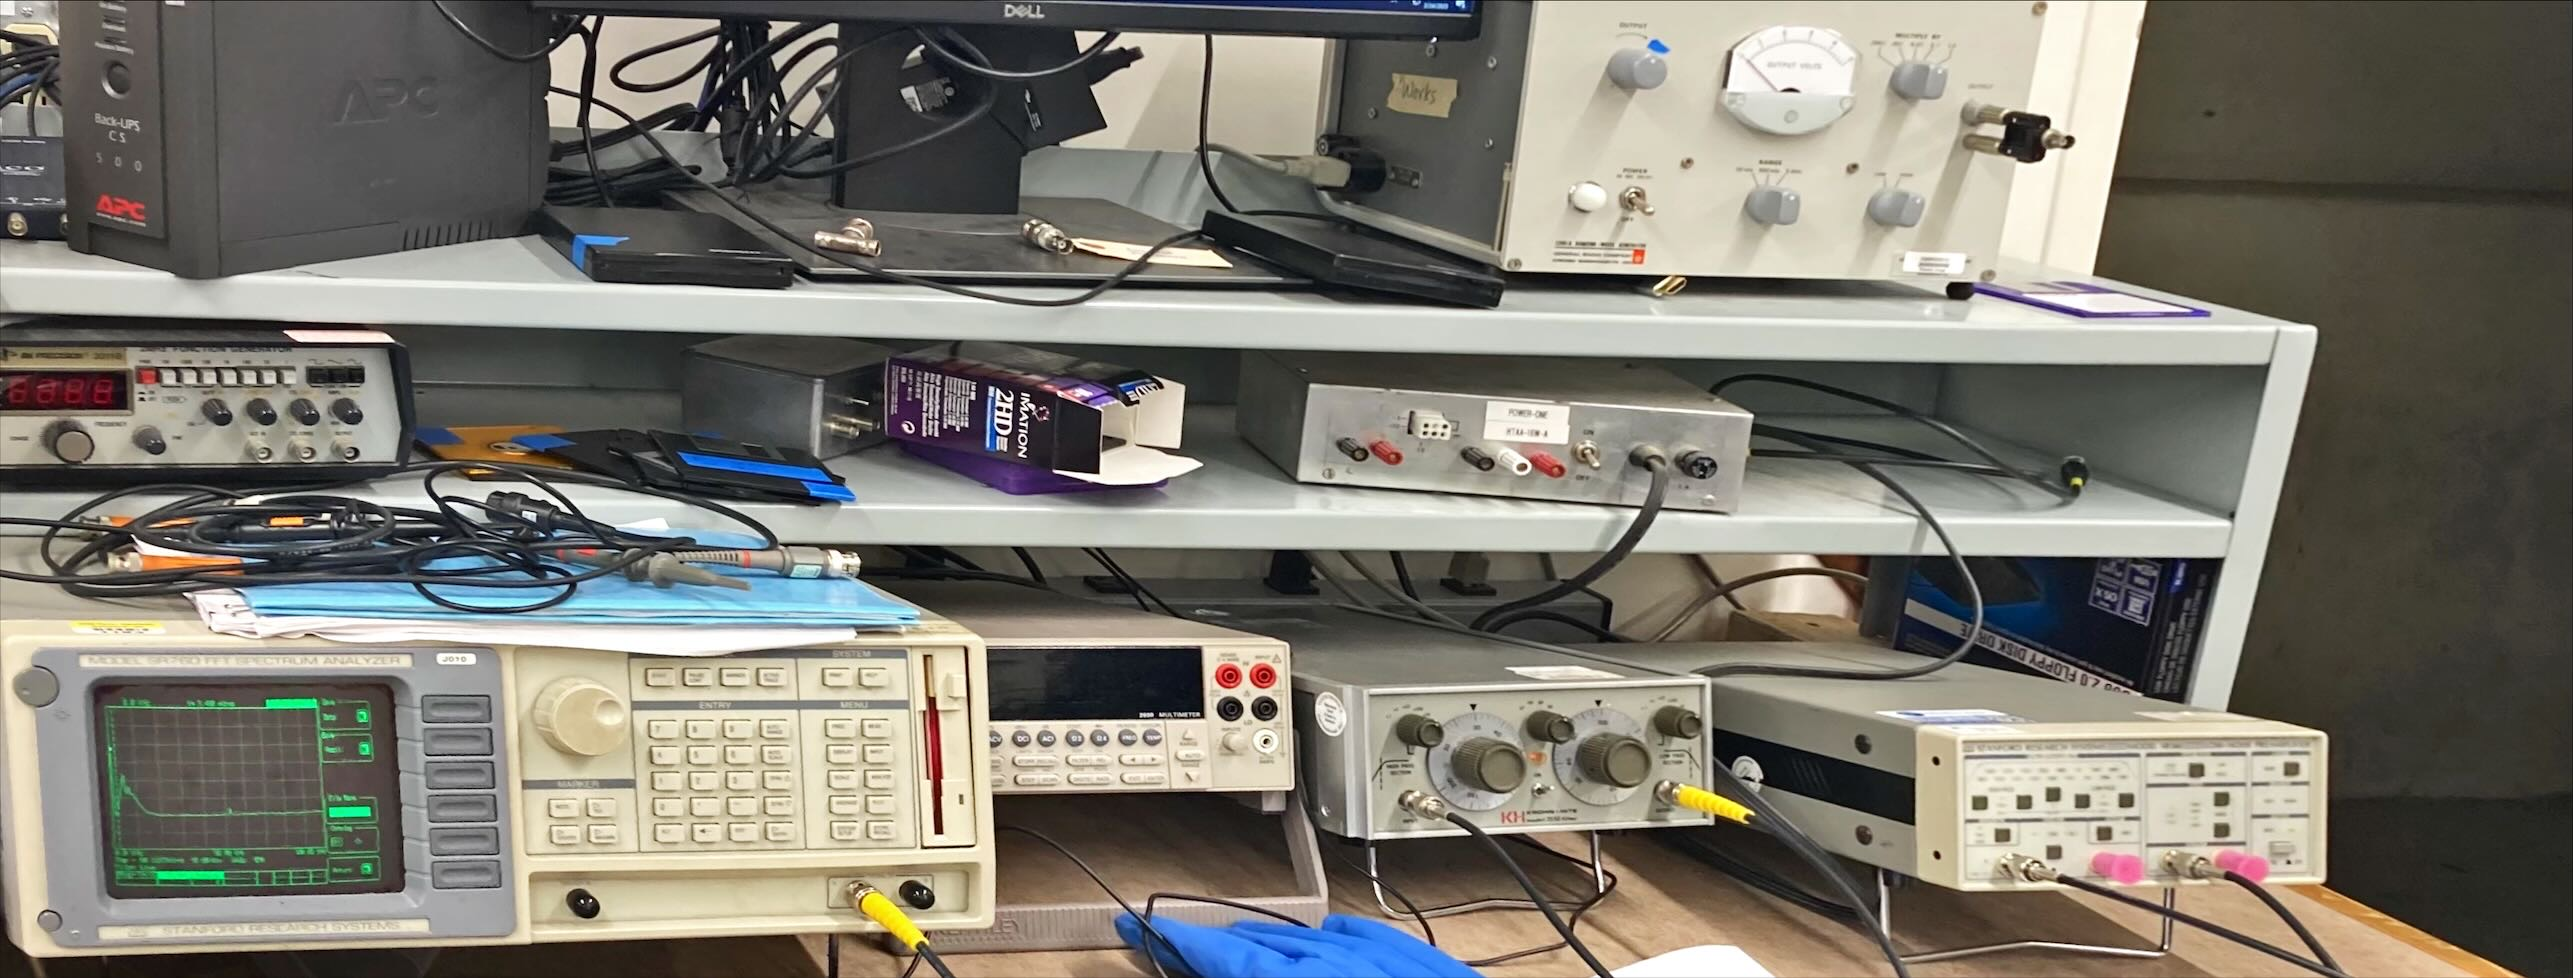
\includegraphics[width= 1 \linewidth]{figures/day1_setup.jpg}
\\
The principle of operation for the cloud chamber involves maintaining evaporated alcohol in a supersaturated state by cooling the bottom plate to a temperature (typically $-35^\circ$ C) at which the vapor pressure is significantly lower than the initial temperature's vapor pressure. This creates a state that favors the transition from vapor to liquid, but due to the polarity of the vapor molecules, this transition is difficult to achieve without free electrons. To address this, the cloud chamber is biased in a manner that restricts the number of free electrons. This allows ionizing radiation to be visible to the naked eye as vapor condensation. In our experiment, we observe the path of condensation created by the alpha particle as it ionizes air and CF4.

Each instance of ionization of the surrounding particles by the alpha particle results in energy loss, which is absorbed by the ionized electron in the form of binding and kinetic energy. The Bethe-Bloch formula describes the energy loss through a medium.

$$-\left<\frac{dE}{dx}\right> = \frac{4\pi}{m_ec^2}\cdot\frac{nz^2}{\beta^2}\cdot\left(\frac{e^2}{4\pi\epsilon_0}\right)^2\cdot\left[\ln\left(\frac{2m_ec^2\beta^2}{I\cdot(1-\beta^2)}\right)-\beta^2\right]$$

\newpage
\section{Result and Analysis}
\subsection{Experiment Result}
In our investigation of $\alpha$-decay using a diffusion cloud chamber, we explored various aspects of this process. Specifically, we examined the relationship between the length and bending angle of $\alpha$-decay trajectories and how different factors impacted the decay rate. The number of $\alpha$-decay traces recorded increased with voltage difference, and we recorded 112 traces in air when the voltage difference was set to $400\pm10$ V, as compared to 66 traces at $100\pm10$ V. This relationship suggests that there is a positive correlation between voltage difference and decay rates, which could be due to higher electron vacancies in regions with greater electrical potential.

However, we observed only 28 traces at $400\pm10$ V in CF$_4$, which is about 25\% of the number of traces observed in air under the same voltage difference. This discrepancy could be due to the vapor pressure of alcohol in different media, indicating that many traces in CF$_4$ are not visible to the naked eye. We also investigated the effect of a nearby gamma ray source on the $\alpha$-decay rate and found no significant difference in the decay rate with or without the gamma ray source. This result may be due to the small size of the target ($\alpha$-decay source), making it difficult for gamma rays to hit it, and resulting in a negligible increase in energy.

Our investigation also revealed that trajectory length varied with the medium but not with the electric potential difference, consistent with our expectations. However, our results for the bending angle had a wider spread than the theoretical prediction for multiple scattering. This could be due to the small sample size and measurement uncertainty. It is worth noting that we used ImageJ to measure trajectory length and bending angle, and the manual alignment of the measuring tool could introduce random error to our data, leading to a wider distribution spread.
\\
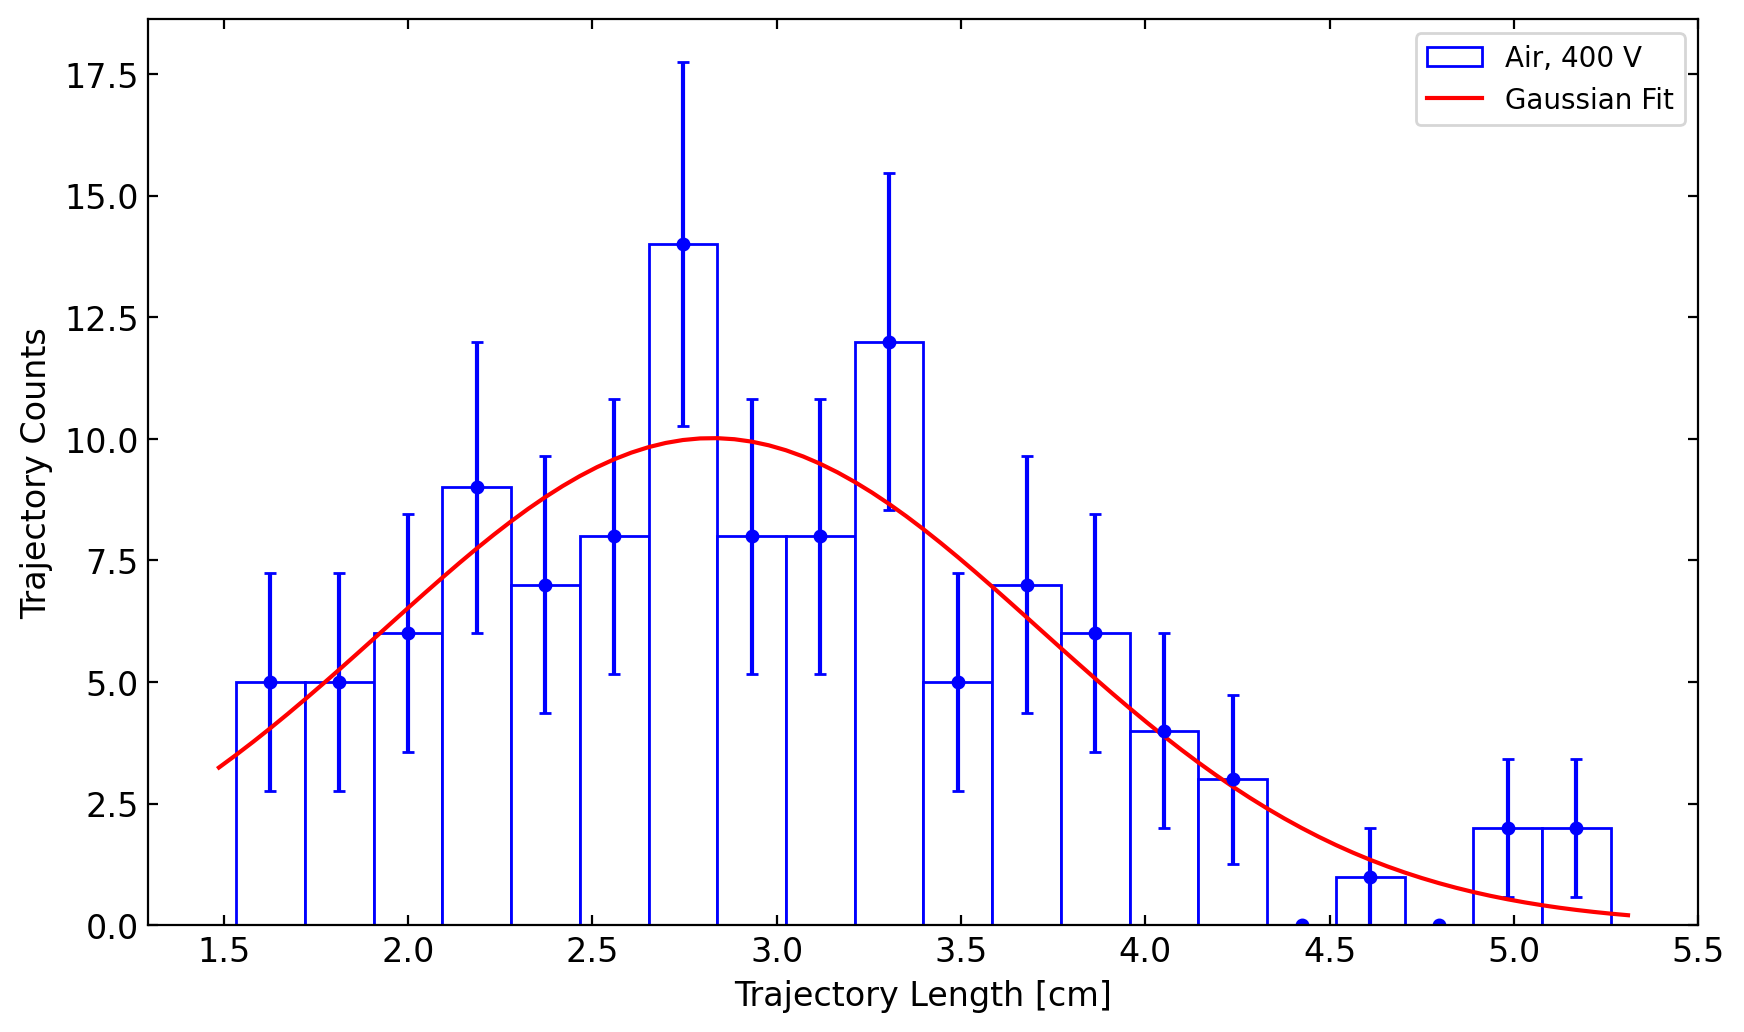
\includegraphics[width = 1\textwidth]{figures/result_air400.png}
\\
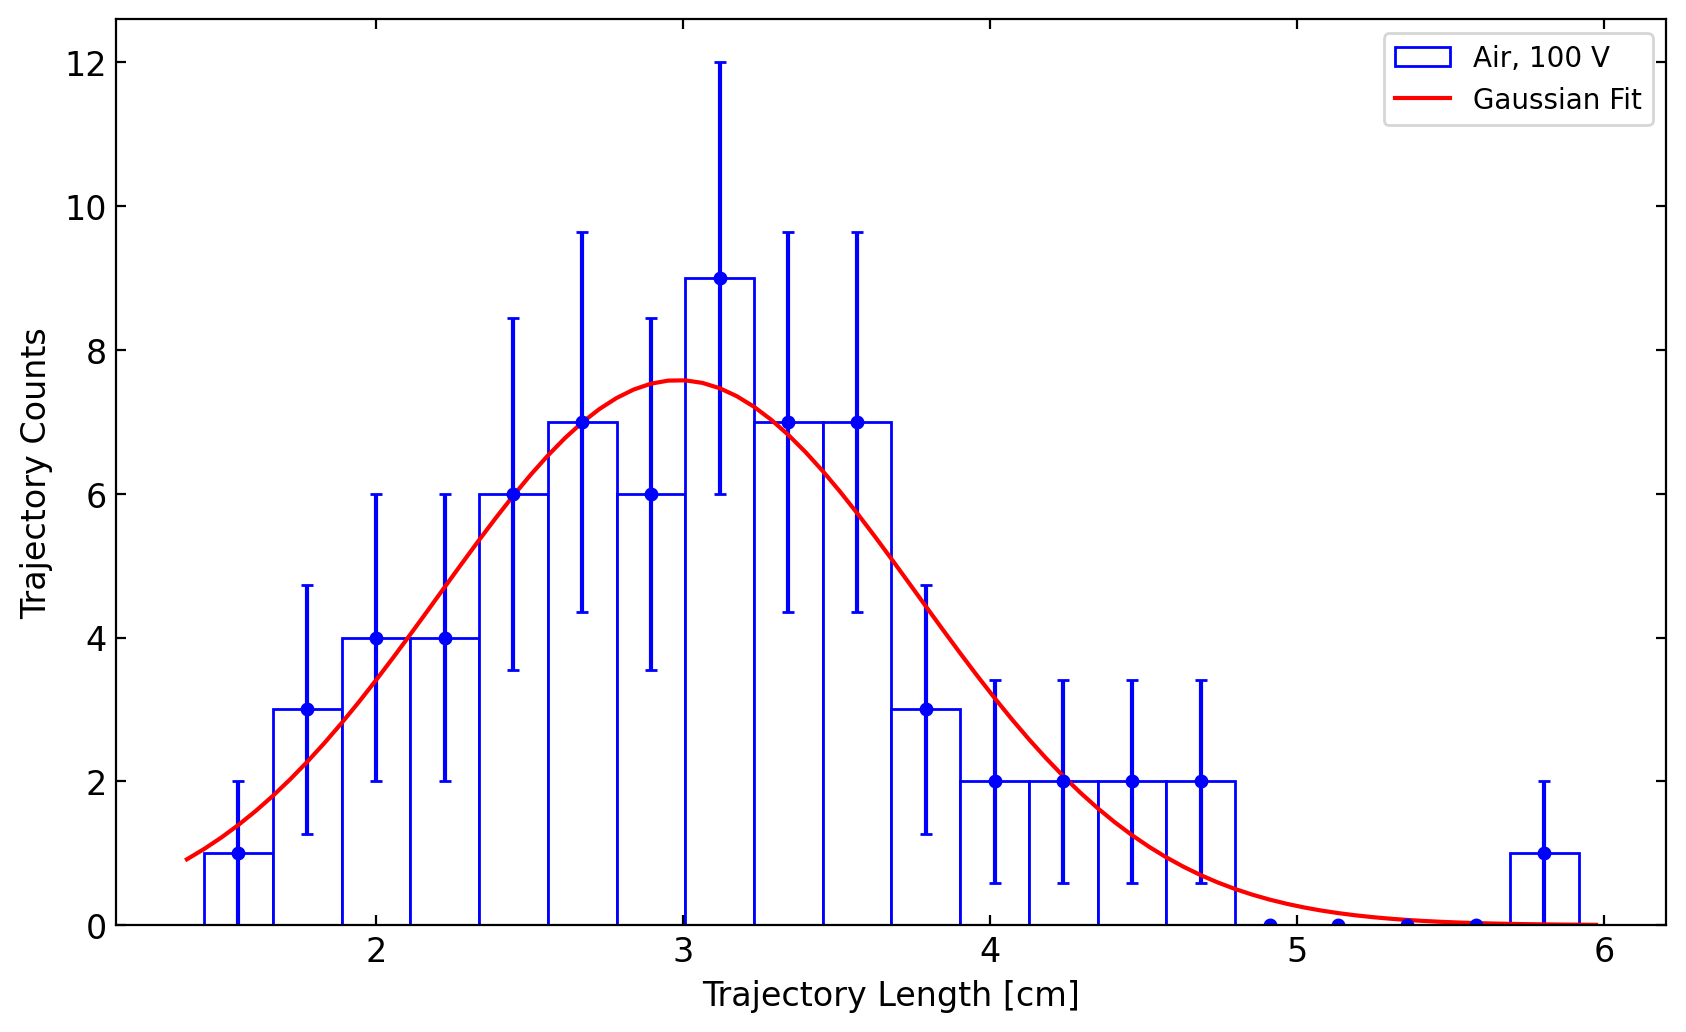
\includegraphics[width = 1\textwidth]{figures/result_air100.png}
\\
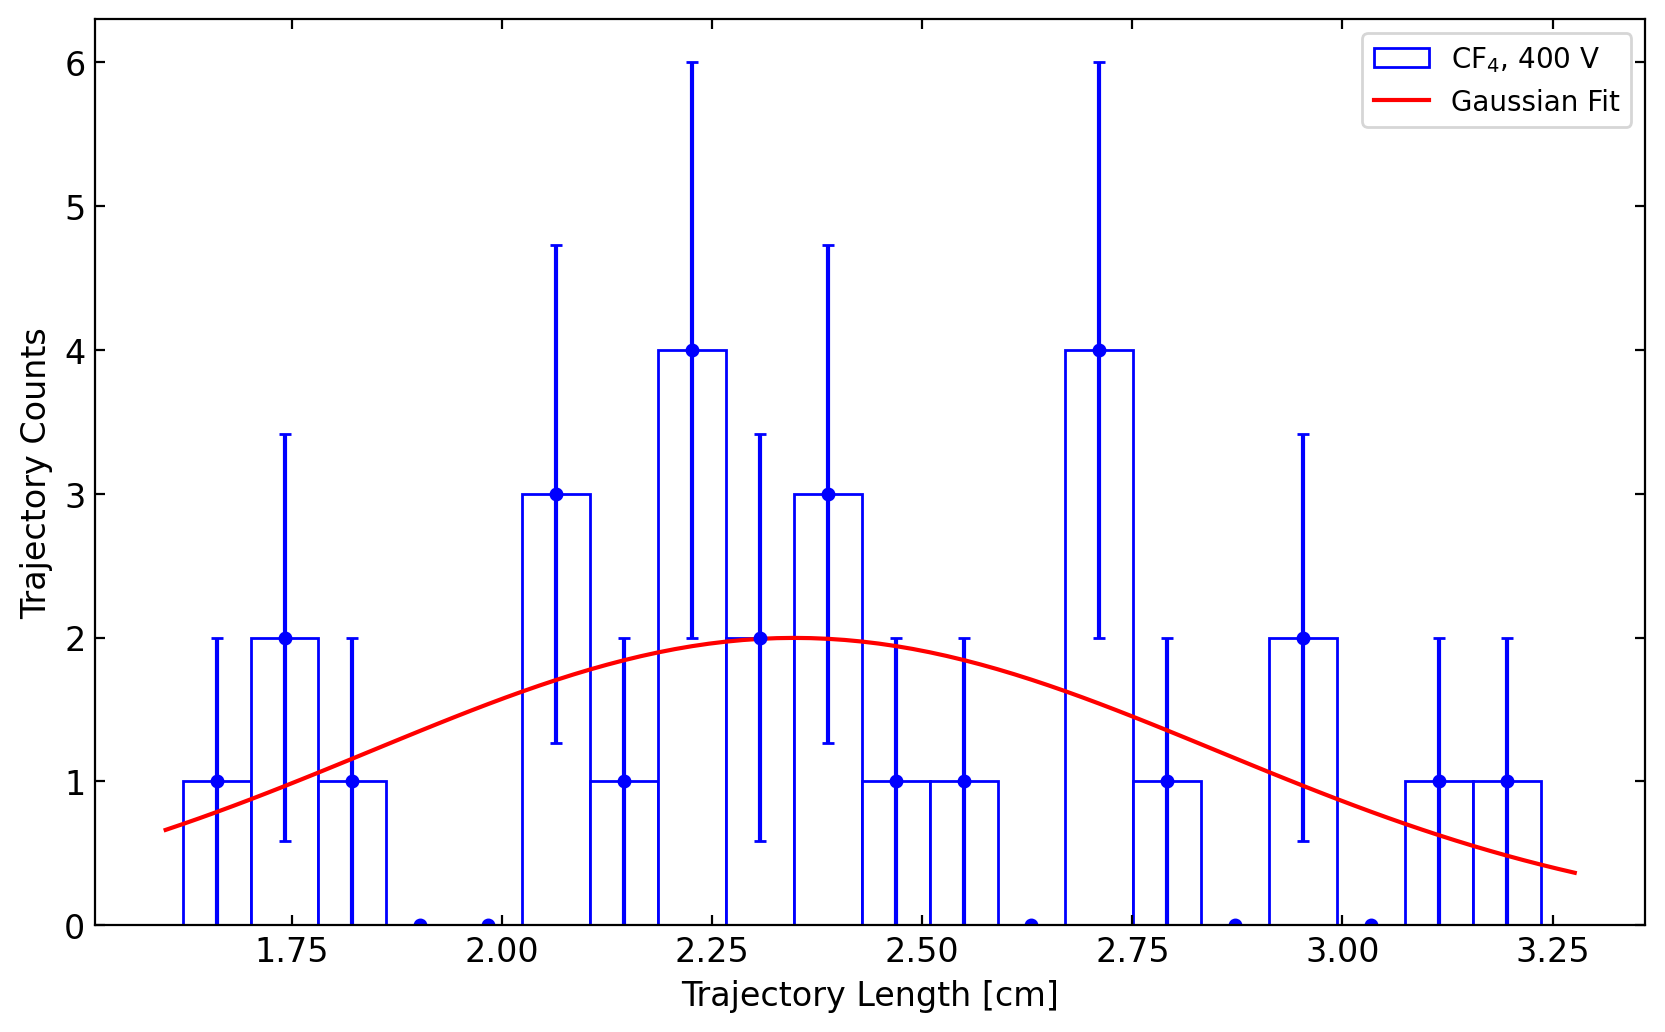
\includegraphics[width = 1\textwidth]{figures/result_cf4400.png}
\\
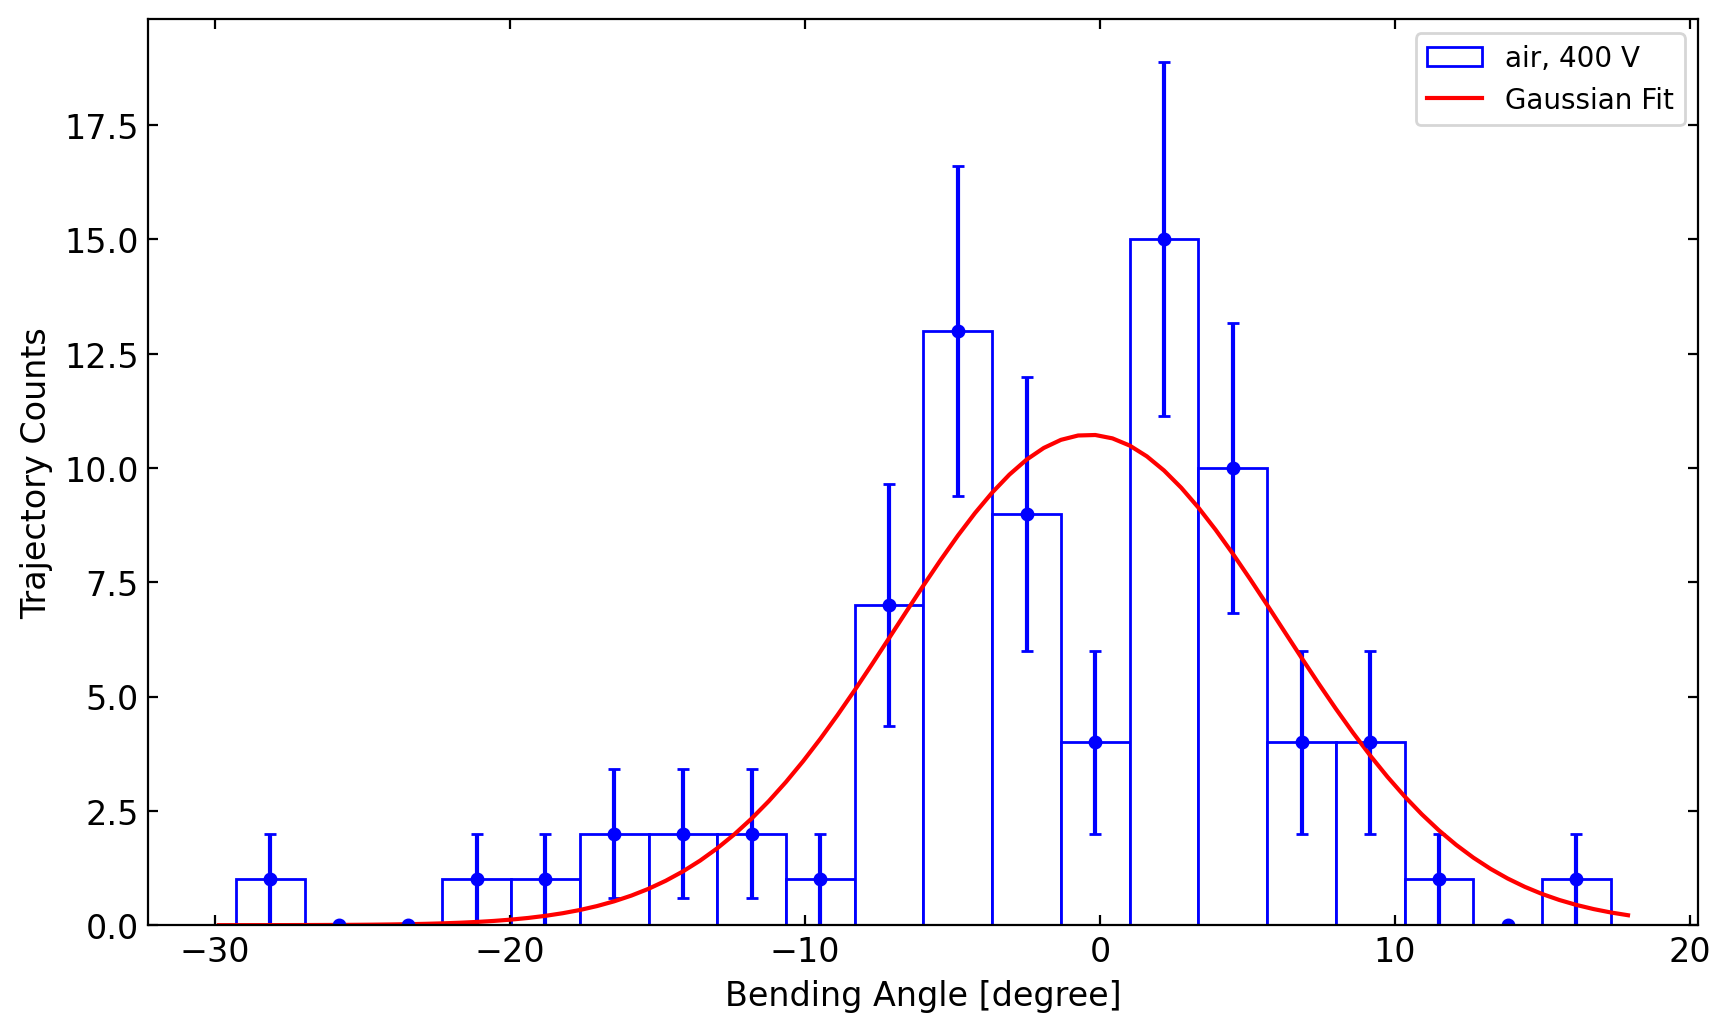
\includegraphics[width = 1\textwidth]{figures/result_scat.png}
\\

\subsection{Qualitative Error Analysis}

In our study of alpha decay using a diffusion cloud chamber, we used ImageJ to measure trajectory length and bending angle. We recognize that manually aligning the measuring tool can introduce random errors to our data, which can widen the distribution spread. We controlled the error for the length measurement to be 10\% or less, as the typical length scale in our measurement was about 2 centimeters. However, for small angle measurements of 2 to 5 degrees, we acknowledge that our data may be off by 50\% or more. This can explain the consistency in length measurement and the discrepancy in angle measurement, as indicated by the large standard deviation after fitting with multiple scattering theory.

We also discovered that our camera was not set at a perfect level, resulting in image distortion. We observed that the distance calibrated as 2 cm near the margin was about 10\% longer than the same distance calibrated near the center. As the trajectory of the alpha particle was bending vertically due to electric potential and gravity, part of the vertical curvature was mapped to the plane of the photo image. Therefore, we may have observed more counterclockwise bending on the upper part of images and more clockwise bending on the lower parts, leading to an overestimation of the spread of the bending angle distribution.

Another source of error was related to the fluidity of the alcohol cloud. The trajectory pointing up near the radioactive source did not seem to be coming directly from the center of the concentric circles. We observed a shift in the trajectory's initial location in our original video file, indicating convection of gas and cloud inside the chamber. This fluid-like convection can be hard to predict, and the trajectory shown in our selected frames may have been distorted by it. To reduce the impact of these errors, we suggest repeating the measurements several times using computer programs to increase data acquisition efficiency and upgrading our photographing setup to solve the camera tilting problem.




\newpage
\section{Discussion}

In this study, we investigated various properties of alpha decay utilizing a diffusion cloud chamber. Our results showed that the trajectory length of alpha particles in air was measured to be $2.82\pm 0.89$ cm, while in CF$_4$, it was found to be $2.35 \pm 0.50$ cm. We observed an increase in the decay rate upon increasing the voltage difference, while the presence of a nearby gamma ray source did not have a significant effect.

Moreover, we estimated the average bending angle of the trajectories to be $-0.38\pm 6.55$ degrees, which could not be fully explained by multiple scattering. We discussed possible sources of error in our length and angle measurements that could have contributed to this discrepancy.

To mitigate the aforementioned errors, we propose some solutions. Firstly, to reduce random error in manual length and angle measurements, we suggest repeating measurements several times. However, this may be challenging to accomplish manually, so implementing a computer program could enhance data acquisition efficiency. Secondly, we suggest upgrading our photographing setup or calculating the offset to improve camera calibration and address any tilting issues. Lastly, we propose identifying the frames with the formation moment of trajectories to mitigate the effect of gas convection. Again, utilizing computer programs may increase measurement efficiency and enable us to perform such tasks with greater accuracy.


%\hrulefill

%%%%%%%%%%%%%%%%%%%%%%%%%%%%%%%%%%%%%%%%%%%%%%%%%%%%%%%%

%\newpage
% \bibliographystyle{plain}
% \bibliography{lab_notes}

\end{document}